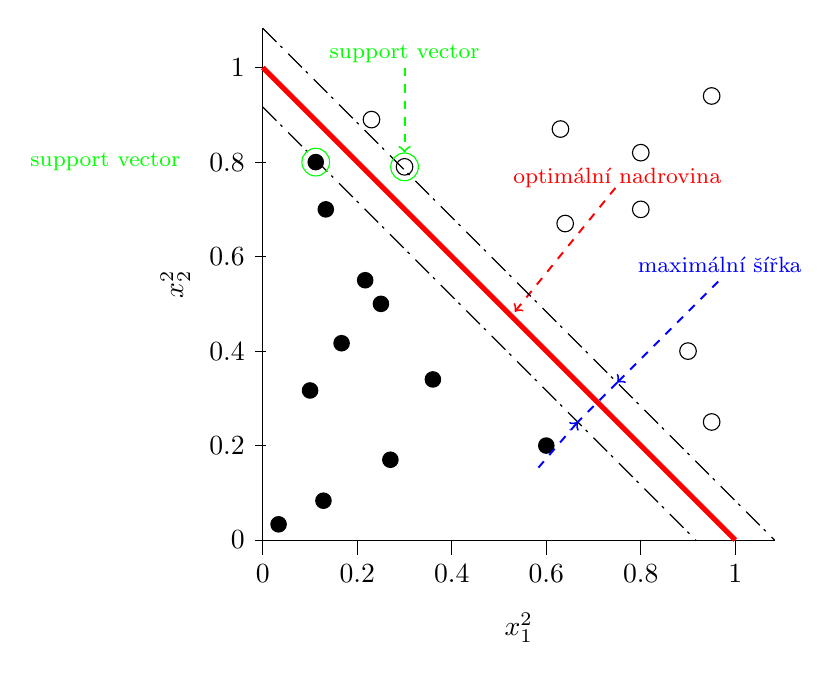
\begin{tikzpicture}
\def\offset{6}
\tikzstyle{redone} = [red,font=\footnotesize,inner sep=1pt]
\tikzstyle{greenone} = [green,font=\footnotesize,inner sep=1pt]
\tikzstyle{blueone} = [blue,font=\footnotesize,inner sep=1pt]
  %axis
  \draw (0,0) -- coordinate (x axis mid) (\offset+0.5,0);
  \draw (0,0) -- coordinate (y axis mid) (0,\offset+.5);
      %ticks 
      \foreach \x in {0,0.2,0.4,0.6,0.8,1}
      \draw (\x*\offset,.2pt) -- (\x*\offset,-5.3pt)
      node[anchor=north] {\x};
      \foreach \y in {0,0.2,0.4,0.6,0.8,1}
      \draw (1pt,\y*\offset) -- (-3pt,\y*\offset)
      node[anchor=east] {\y}; 
  %labels      
  \node[below=0.8cm] at (x axis mid) {$x_1^2$};
  \node[rotate=90, above=0.8cm] at (y axis mid) {$x_2^2$ };
  %coord
  \draw[arrows=<-,line width=0.7pt, dashed,red](3.2,2.9)--(4.5,4.5);
  \node[redone] at (4.5,4.6) {optimální nadrovina};
    %points negative
    \fill[black] (1,2.5)     circle (3pt);
    \fill[black] (0.2,.2)    circle (3pt);
    \fill[black] (0.6,1.9)   circle (3pt);
    \fill[black] (0.77, 0.5) circle (3pt);
    \fill[black] (1.5,3)     circle (3pt);
    \fill[black] (1.3,3.3)   circle (3pt);
    \fill[black] (0.8,4.2)   circle (3pt);
    \fill[black] (0.6*\offset, \offset *0.2)   circle (3pt);
    \fill[black] (0.36*\offset, \offset *0.34)   circle (3pt);
    \fill[black] (0.27*\offset, \offset *0.17)   circle (3pt);
      \fill[black] (\offset*0.112, \offset*0.8)   circle (3pt); %on line
      %points positive
      \draw (0.8*\offset, \offset *0.7)   circle (3pt);
      \draw (0.8*\offset, \offset *0.82)   circle (3pt);
      \draw (0.9*\offset, \offset *0.40)   circle (3pt);
      \draw (0.64*\offset, \offset *0.67)   circle (3pt);
      \draw (0.95*\offset, \offset *0.94)   circle (3pt);
      \draw (0.3*\offset, \offset *0.79)   circle (3pt); % on line
      \draw (0.23*\offset, \offset *0.89)   circle (3pt);
      \draw (0.63*\offset, \offset *0.87)   circle (3pt);
      \draw (0.95*\offset, \offset *0.25)   circle (3pt);
      %svm lines
  \draw[line width=0.65mm, red] (0,\offset) -- (\offset,0);
  \draw[line width=0.15mm,dash pattern={on 7pt off 2pt on 1pt off 3pt}] (0,\offset-0.5) -- (\offset-0.5,0);
  \draw[line width=0.15mm,dash pattern={on 7pt off 2pt on 1pt off 3pt}] (0,\offset+0.5) -- (\offset+0.5,0);
  %arrow supp vectors
      \draw[greenone] (0.3*\offset, \offset *0.79)   circle (5pt); % on positive
      \draw[greenone] (\offset*0.112, \offset*0.8)   circle (5pt); % on negative
%      \draw[arrows=->,line width=0.7pt, dashed,green](-1,\offset*0.8)--(\offset*0.08, \offset*0.8);
      \node[greenone] at (-2,\offset*0.8) {support vector};
      \draw[arrows=->,line width=0.7pt, dashed,green](0.3*\offset, \offset )--(0.3*\offset, \offset *0.82);
      \node[greenone] at (0.3*\offset, \offset*1.03) {support vector};
%    %maximum width
    \draw[arrows=<-,line width=0.7pt, dashed,blue](4.5,2)--(5.8,3.3);
    \draw[arrows=-,line width=0.7pt, dashed,blue](4.5,2)--(3.9,1.4);
    \draw[arrows=->,line width=0.7pt, dashed,blue](3.5,0.92)--(4,1.5);
    \node[blueone] at (5.8,3.5) {maximální šířka};
 \end{tikzpicture}